\documentclass[fontsize=12pt, toc=bibliography, notitlepage]{scrreprt}

\usepackage[ngerman]{babel}
\usepackage{ucs}
\usepackage[utf8x]{inputenc}
\usepackage[bookmarksopen=true,
			bookmarks=true,
			plainpages=false,
        	pdfpagelabels=true,
			colorlinks=true,
			linkcolor=black,
			citecolor=black,
        	filecolor=black,
        	urlcolor=blue]{hyperref}
\usepackage{graphicx}
\usepackage{float}
\usepackage{listings}
\usepackage{color}
\usepackage{tikz}
\usepackage[Q=yes]{examplep}
\usepackage[hypcap]{caption}

\title{Jefax}
\subtitle{Ein Kernel für Atmels XMega}
\author{Fabian Meyer \and Jens Gansloser}
\date{\today \\ HTWG Konstanz}

\lstdefinestyle{MyCStyle}{
  belowcaptionskip=1\baselineskip,
  breaklines=true,
  frame=single,
  captionpos=b,
  numbers=left,
  xleftmargin=\parindent,
  language=C,
  showstringspaces=false,
  basicstyle=\footnotesize\ttfamily,
  keywordstyle=\bfseries\color{green!40!black},
  commentstyle=\itshape\color{purple!40!black},
  identifierstyle=\color{blue},
  stringstyle=\color{orange}
}
\lstset{escapechar=@,style=MyCStyle}

\newcommand{\refnn}[1]{\ref{#1} \nameref{#1}}

\begin{document}

\maketitle

\begin{abstract}
Jefax ist ein einfacher Betriebssystemkernel, der preemptives Scheduling und damit Multitasking realisiert. Zusätzlich sind einfache Synchronisierungsmechanismen wie Mutex und Condition Variable implementiert. Die dynamische Speicherverwaltung erlaubt die Entwicklung flexibler Datenstrukturen und Tasks. Über die serielle UART Schnittstelle ist eine Shell zur Ausgabe von ASCII Strings verfügbar.
\end{abstract}
\clearpage

\tableofcontents

\chapter{Tasks}
\label{chap:tasks}
Wie in einem Multitasking-Betriebssystem üblich, können vom Benutzer verschiedene Tasks erzeugt werden, die vom Scheduler geschedult werden. Intern werden Tasks für den Dispatcher sowie optional für die Shell verwendet. Jede Tasks besitzt ihren eigenen Task-Kontext. Bei einem Kontextwechsel wird dieser gesichert bzw. wiederhergestellt. Verschiedene Schedulingverfahren erlauben das quasi-parallele Ausführen der Tasks.\\

\begin{lstlisting}[title=task.h]
typedef struct {
	int (*function)();

	unsigned int priority;
	volatile taskState_t state;

	uint8_t *stackpointer;

	uint8_t stack[STACK_SIZE];
} task_t;
\end{lstlisting}

Eine Task wird durch die Struktur \lstinline$task_t$ repräsentiert. Diese besteht aus:

\begin{itemize}
\item Pointer auf die Task Funktion
\item Priorität der Task
\item Taskstatus (READY, RUNNING, BLOCKING)
\item Stackpointer, der auf die nächste freie Speicheradresse auf dem Stack zeigt.
\item Ein Feld von \lstinline$uint8_t$, welches den Stack darstellt.
\end{itemize}

Der Stack besitzt zur Laufzeit eine feste Größe, welche durch das Symbol \lstinline$STACK_SIZE$ festgelegt werden kann. Dieses Symbol kann zur Kompilierzeit definiert werden, ansonsten wird ein Standardwert verwendet. Wichtig zu wissen ist hierbei, dass der Stack sich nicht im Compiler-spezifischen Stackbereich befindet (Stack-Section - beginnend von der letzten Adresse im SRAM), sondern in der Data-Section.

\section{API}
\label{subsec:tasks-api}
Zum Erzeugen einer Task wird die Funktion \lstinline$initTask()$ verwendet. Aufgabe dieser Funktion ist es, den Stack sowie den Stackpointer zu initialisieren. Der Funktionspointer der Taskfunktion muss vor dem Aufruf von \lstinline$initTask()$ gesetzt werden.

\begin{lstlisting}
void initTask(task_t *task);
\end{lstlisting}

Um zu bestimmen, welche Tasks geschedult werden sollen, wird das Feld \lstinline$TASKS$ in \lstinline$jefax.c$ verwendet. Ein Benutzer kann hier die zu schedulenden Tasks eintragen. Als letztes Element in dem Feld muss sich immer ein leeres \lstinline$task_t$ Element befinden. Optional kann das Makro \lstinline$SHELL_TASK$ zum aktivieren der Shell verwendet werden.

\begin{lstlisting}[title=jefax.c]
task_t TASKS[] = {
    {counterTask2, 2, READY, 0, {0}},
    SHELL_TASK,
    {0, 0, READY, 0, {0}}
};
\end{lstlisting}

Ein Eintrag im \lstinline$TASKS$ Feld besteht aus:

\begin{itemize}
\item Pointer auf die Task-Funktion
\item Priorität der Task
\item Initialer Status der Tasks (meist READY)
\item Stackpointer (muss immer 0 sein)
\item Stack (muss immer {0} sein)
\end{itemize}

\section{Implementierung}
\label{subsec:tasks-impl}
Da bei den XMega Microcontrollern der Stack von der höchsten zur niedrigsten Adresse wächst, wird der Stackpointer mit

\begin{lstlisting}
task->stackpointer = task->stack + STACK_SIZE - 1;
\end{lstlisting}

initialisiert. Anschließend wird die Adresse der Task Funktion auf dem Stack abgelegt (bei den XMega128 3 Byte). Zuletzt werden noch die 32 Arbeitsregister sowie das Statusregister auf dem Stack benötigt.

Damit auch andere Komponenten (z.B. Scheduler) auf die globale \lstinline$TASKS$ Struktur zugreifen können, wird dieses Feld in den jeweiligen Dateien als extern deklariert.

\begin{lstlisting}
extern task_t TASKS[];
\end{lstlisting}

\chapter{Scheduling}
\label{chap:scheduling}
Essentieller Bestandteil von Jefax ist das Scheduling. Die Tasks im Kernel laufen preemptiv, d.h. sie können unterbrochen und ausgewechselt werden. Um einen sicheren quasiparallelen Ablauf zu garantieren, muss beim Austausch der Tasks deren Kontext gesichert werden (siehe \refnn{sec:dispatcher}.\\
Die 2 Kernbestandteile des Scheduling sind der Dispatcher und der Scheduler. Der Standardscheduler realisiert ein prioritätengesteuertes Round-Robin-Verfahren. Tasks werden können durch höherpriore Tasks unterbrochen und verdrängt werden. Haben die mehrere Tasks die gleiche Priorität, erhalten sie reihum eine feste Zeitscheibe, in der sie Zugriff auf die CPU erhalten. Ist diese Zeitscheibe abgelaufen, werden sie durch den Dispatcher unterbrochen und ausgewechselt.

\section{Dispatcher}
\label{sec:dispatcher}
Der Dispatcher übernimmt das Auswechseln und unterbrechen der Tasks. Das zentrale Element des Dispatchers ist ein Timerinterrupt, der in Regelmäßigen Abständen zuschlägt. Er sichert den Kontext der unterbrochenen Task und wechselt eine andere Task wieder ein.

\subsection{API}
\label{subsec:dispatcher-api}

Die Zeitscheibe nach der der Dispatcher zuschlägt kann zur Laufzeit durch den Aufruf der Funktion 

\begin{lstlisting}
void setInterruptTime(unsigned int p_msec);
\end{lstlisting}

gesetzt werden. Die Funktion bietet eine Auflösung im Millisekundenbereich.

\subsection{Implementierung}
\label{subsec:dispatcher-impl}
Bevor der Dispatcher genutzt werden kann muss die Funktion

\begin{lstlisting}[title=dispatcher.c]
void initDispatcher()
{
	initScheduler(getRRScheduler());
	
	init32MHzClock();
	initUsart();
	initTimeSliceTimer();
	
	// Save the main context
	SAVE_CONTEXT();
	main_stackpointer = (uint8_t *) SP;
	
	SP = (uint16_t) (getRunningTask()->stackpointer);
	enableInterrupts();
	RESTORE_CONTEXT();
	
	RET();
}
\end{lstlisting}

aufgerufen werden. Diese Funktion initialisiert den Standardscheduler (Zeile 3, siehe \refnn{subsec:scheduler-impl}), die Taktfrequenz des Prozessors (Zeile 5), die UART-Schnittstelle (Zeile 6) und den Timer, der die Dispatcher Interrupts auslöst (Zeile 7). Danach wird der aktuelle Kontext gespeichert und der Stackpointer als Systemstack gesichert (Zeile 10 - 11). Der Systemstack wird für Interruptserviceroutinen innerhalb von Jefax verwendet.\\
Nun wird der Kontext auf denjenigen der vom Scheduler ausgewählten Task (\lstinline$getRunningTask()$, Zeile 13) gewechselt.\\
Erst jetzt (Zeile 15, \lstinline$enableInterrupts()$) werden die Interrupts global aktiviert. Der Grund hierfür ist, dass sämtliche ISRs in Jefax den Kontext der aktuell laufenden Task sichern. Das bedeutet, dass zu jedem Zeitpunkt, an dem ein Interrupt den Programmfluss unterbrechen kann, eine Task laufen muss. Die ISRs in Jefax werden durch das folgende Makro definiert:

\begin{lstlisting}[title=interrupt.h]
#define JEFAX_ISR(vect, func)								\
ISR(vect, ISR_NAKED)										\
{															\
	SAVE_CONTEXT();											\
	getRunningTask()->stackpointer = (uint8_t *) SP;		\
	ENTER_SYSTEM_STACK();									\
	func();													\
	SP = (uint16_t) (getRunningTask()->stackpointer);		\
	RESTORE_CONTEXT();										\
	reti();													\
}
\end{lstlisting}

Dem Makro \lstinline$JEFAX_ISR()$ muss als erster Parameter der Interruptvektor übergeben werden, der behandelt werden soll. Der zweite Parameter ist eine Funktion, die vorzugsweise vom Typ \lstinline$void (*func)(void)$ sein sollte. Diese Funktion sollte die Behandlung des Interrupts beinhalten. Die \lstinline$JEFAX_ISR()$ sichert beim Auftritt des Interrupts den Kontext der aktuell laufenden Task und deren Stackpointer (Zeile 4 - 5). Danach wird der Systemstack betreten (Zeile 6). Alle ISR in Jefax arbeiten auf dem Systemstack. Nun wird die übergebene Funktion ausgeführt (Zeile 7).\\
Am Ende wird der Kontext der aktuellen Task wieder hergestellt und zu dieser zurückgesprungen (Zeile 8 - 9).\\
Das Sichern des Kontext (\lstinline$SAVE_CONTEXT()$) umfasst lediglich das Ablegen aller CPU-Register sowie das SREG auf dem Stack der Task. \lstinline$RESTORE_CONTEXT()$ macht genau das Gegenteil und lädt die Register vom Stack.\\
Der Dispatcher behandelt Timerinterrupts mit einer \lstinline$JEFAX_ISR()$. Hiermit werden die Tasks unterbrochen und ausgewechselt.

\begin{lstlisting}[title=dispatcher.c]
JEFAX_ISR(TCC0_OVF_vect, schedule)
\end{lstlisting}

Im Rahmen dieser ISR wird der Scheduler aufgerufen um eine neue Task auszusuchen, die laufen soll (dazu mehr in \refnn{subsec:scheduler-impl}.

\newpage

\section{Scheduler}
\label{sec:scheduler}
Der Scheduler des Kernels entscheidet welche der vorhandenen Tasks als nächstes eingewechselt werden soll. Daher ist er entscheidend für das Verhalten des Taskschedulings und auch dessen Performance. Als Standardschedulingverfahren wird in Jefax ein prioritätengesteuertes Round-Robin-Verfahren verwendet.

\subsection{API}
\label{subsec:scheduler-api}
Der Scheduler kann zur Laufzeit mit der Funktion

\begin{lstlisting}
void setScheduler(scheduler_t *p_scheduler);
\end{lstlisting}

geändert werden. In Jefax wird der Scheduler durch die Struktur \lstinline$scheduler_t$ repräsentiert.

\begin{lstlisting}[title=scheduler.h]
typedef struct
{
	void (*init)();
	task_t* (*getNextTask)();
	void (*taskStateChanged)(task_t*);
	void (*taskWokeUp)(task_t*);
	taskList_t *readyList;
	taskList_t *blockingList;
} scheduler_t;
\end{lstlisting}

Um einen selbstimplementierten Scheduler in Jefax zu nutzen, müssen die Callback Funktionen der Struktur implementiert werden. Die Funktion \lstinline$init()$ wird aufgerufen, sobald der Scheduler als neuer Scheduler des Kernels bestimmt wurde. Dabei müssen vor allem die \lstinline$readyList$ und die \lstinline$blockingList$ so bearbeitet werden, dass der Scheduler mit den Listen richtig arbeiten kann.\\

Die Funktion \lstinline$getNextTask()$ wird vom indirekt durch den Dispatcher im Rahmen des Timerinterrupts aufgerufen (siehe \refnn{subsec:dispatcher-impl}). Damit läuft diese Funktion im Interruptkontex. Es dürfen also keine Aufrufe gemacht werden, die zum Schlafen führen könnten (z.B. \lstinline$lockMutex()$). Die Aufgabe dieser Funktion ist es zu bestimmen, welche Task als nächstes eingwechselt werden soll. Als Rückgabewert wird die einzuwechselnde Task erwartet oder \lstinline$NULL$, wenn keine Task gefunden wurde. Wird \lstinline$NULL$ zurückgegeben wechselt Jefax die sogenannte idleTask ein, die nichts macht und als Dummy dient.\\

Mit dem Callback \lstinline$taskStateChanged(task_t*)$, wird dem Scheduler signalisiert, dass eine Task ihren Zustand geändert hat. Der Scheduler sollte entsprechend auf diese Änderung reagieren, z.B. die aktuelle Task verdrängen falls eine höherpriore Task rechenbereit wurde. Als Parameter wird die Task übergeben, deren Zustand sich verändert hat.\\

Der Aurfruf von \lstinline$taskWokeUp(task_t*)$ scheint auf den ersten Blick dem Aufruf von \lstinline$taskStateChanged(task_t*)$ sehr zu ähneln. Jedoch gibt es einen bedeutenden Unterschied: \lstinline$taskWokeUp(task_t*)$ läuft im Interrupt Kontext, es darf also nicht auf den nächsten Timerinterrupt gewartet werden (z.B. durch schlafen, yield, etc). Hier ist die übergebene Task diejenige, die aufgewacht ist.\\

Die beiden Listen \lstinline$readyList$ und \lstinline$blockingList$ werden gesetzt, sobald der Scheduler mithilfe von \lstinline$setScheduler(scheduler_t*)$ als neuer Scheduler bestimmt wird. Sie beinhalten die Tasks, die den der Liste entsprechenden Zustand haben.\\
Auf die aktuell laufende Task kann mit der Funktion

\begin{lstlisting}
task_t *getRunningTask();
\end{lstlisting}

zugegriffen werden.\\

Der Status einer Task (\lstinline$RUNNING$, \lstinline$BLOCKING$, \lstinline$READY$) kann über die Funktion

\begin{lstlisting}
void setTaskState(task_t *p_task, taskState_t p_state);
\end{lstlisting}

geändert werden.\\
Alternativ können die Funktionen \lstinline$yield()$ und \lstinline$void sleep(const int p_ms)$ verwendet werden, um Task in den Zustand \lstinline$READY$ bzw. \lstinline$BLOCKING$ zu überführen.
Die Funktion \lstinline$int hasRunningTask()$ erlaubt die Überprüfung, ob momentan eine Task läuft. Dies ist genau dann der Fall, wenn nicht die \lstinline$idleTask$ läuft.
Mit \lstinline$void forceContextSwitch()$ kann ein Kontextswitch, also eine Unterbrechung der aufrufenden Task erzwungen werden.

\subsection{Implementierung}
\label{subsec:scheduler-impl}
Bevor der Scheduler genutzt werden kann muss die Funktion

\begin{lstlisting}
int initScheduler(scheduler_t *p_defaultScheduler)
{
	int ret;
	initTask(&idleTask);
	
	ret = initTaskLists();
	if(ret)
		return ret;
		
	ret = initTimerSystem();
	if(ret)
		return ret;
		
	setScheduler(p_defaultScheduler);
	setFirstRunningTask();
	
	return 0;
}
\end{lstlisting}

ausgeführt werden. Diese wird im Rahmen von \lstinline$initDispatcher$ aufgerufen. Zuerst wird die \lstinline$idleTask$ initialisiert (Zeile 4). Danach werden die Tasklisten, als die \lstinline$readyList$ und die \lstinline$blockingList$ initialisiert (\lstinline$ret = initTaskLists()$, Zeile 8). Im Rahmen dieser Funktion wird die \lstinline$readyList$ mit den Tasks aus dem \lstinline$TASKS$ Feld gefüllt.\\
Daraufhin wird das Timersystem initialisiert, welches für den Aufruf von \lstinline$sleep()$ benötigt wird.\\
Zuletzt wird der Standardscheduler gesetzt und die erste Task ausgewählt, die geschedult werden soll (Zeile 14 - 15).\\

Die zentrale Funktion des Schedulers, die auch vom Dispatcher (siehe \refnn{subsec:dispatcher-impl}) aufgerufen wird, \lstinline$schedule()$ ist folgender Maßen implementiert:

\begin{lstlisting}[title=scheduler.c]
void schedule()
{
	runningTask = scheduler->getNextTask();
	// no task was found, so schedule idleTask
	if(runningTask == NULL)
		runningTask = &idleTask;
	runningTask->state = RUNNING;
}
\end{lstlisting}

Zuerst wird die nächste Task durch den Aufruf des Callbacks \lstinline$getNextTask()$ des aktuellen Schedulers ausgewählt (Zeile 3). Die Variable \lstinline$runningTask$ ist dabei global definiert und stellt die aktuell laufende Task dar.\\

In Zeile 5 wird überprüft, ob der Scheduler eine lauffähige Task gefunden hat. Dies wird durch den Rückgabewert \lstinline$NULL$ des Callbacks signalisiert. Wird keine Task gefunden, wird die sogenannte \lstinline$idleTask$ als \lstinline$runningTask$ ausgewählt.\\

Beim Ändern des Taskzustands wird folgender Code ausgeführt:

\begin{lstlisting}[title=scheduler.c]
void setTaskState(task_t *p_task, taskState_t p_state)
{
	uint8_t irEnabled = enterAtomicBlock();
	
	p_task->state = p_state;
	scheduler->taskStateChanged(p_task);
		
	exitAtomicBlock(irEnabled);	
}
\end{lstlisting}

Hierbei wird ununterbrechbar (\lstinline$enterAtomicBlock()$) der Zustand der Task geändert (Zeile 5) und danach das Callback des Schedulers (Zeile 6) ausgeführt.\\

Die Funktion \lstinline$void forceContextSwitch()$ hat folgende Implementierung:

\begin{lstlisting}[title=scheduler.c]
void forceContextSwitch()
{
	// save interrupt enable state
	uint8_t state = SREG & 0x80;
	// create interrupt
	sei();
	FORCE_INTERRUPT(TCC0);
	
	// wait to be exchanged
	while(!TASK_IS_RUNNING(runningTask))
	{ }
	
	if(!state)
		cli();
}
\end{lstlisting}

In Zeile 4 wird der aktuelle Zustand des Interruptenablebits gesichert. Danach wird ein Timerinterrupt des Dispatchers erzwungen. Dazu werden Interrupts aktiviert (Zeile 6) und das Makro \lstinline$FORCE_INTERRUPT()$ aufgerufen (Zeile 7). Diese Makro setzt den Counter des Timers auf den Wert kurz vor dem Auslösen des Interrupts. Nun wird in einer Schleife darauf gewartet, dass die Task wieder den Zustand \lstinline$RUNNING$ annimmt (Zeile 10). Dies impliziert, dass vor dem Aufruf von \lstinline$void forceContextSwitch()$ der Zustand der Task auf einen anderen Zustand als \lstinline$RUNNING$ gesetzt wurde.

\subsection{Zustandsautomat}
\label{subsec:zustandsautomat}
In Jefax gibt es 3 Taskzustände: \lstinline$READY$, \lstinline$RUNNING$, \lstinline$BLOCKING$. Der Übergang zwischen diesen Zuständen wird in \autoref{fig:zustandsautomat} dargestellt.

\begin{figure}[H]
	\centering
	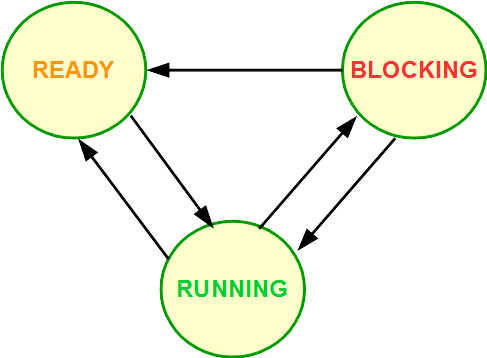
\includegraphics[width=200px]{images/Zustandsautomat.png}
	\caption{Zustandsautomat}
	\label{fig:zustandsautomat}
\end{figure}

Alle Tasks starten initial mit dem Zustand \lstinline$READY$. Aus diesem Zustand heraus können die Tasks nur in den Zustand \lstinline$RUNNING$ wechseln (siehe \autoref{fig:zustandsautomat}), indem sie vom Scheduler ausgewählt und durch den Dispatcher eingewechselt werden.\\

Aus dem Zustand \lstinline$RUNNING$ kann die Task in die Zustände \lstinline$BLOCKING$ oder \lstinline$READY$ wechseln, je nach dem welche Ereignisse zur Laufzeit auftreten. Von \lstinline$BLOCKING$ gibt es entweder die Möglichkeit in den Zustand \lstinline$READY$ oder direkt in den Zustand \lstinline$RUNNING$ zu wechseln.\\

Hierbei handelt es sich jedoch nur um eine Empfehlung für die Zustandsänderung. Wie der Zustandsautomat tatsächlich aussieht hängt von der Implementierung der Funktion \lstinline$taskStateChanged()$ (siehe \refnn{subsec:scheduler-api}) des Schedulers ab.

\subsection{Round Robin Scheduler}
\label{subsec:round-robin-scheduler}
Der einzige standardmäßig implementierte Scheduler in Jefax - und damit auch der Defaultscheduler - ist ein prioritätengesteuerter Round-Robin-Scheduler. Dieser kann über die Funktion

\begin{lstlisting}
scheduler_t *getRRScheduler();
\end{lstlisting}

genutzt werden.\\

Der Scheduler implementiert sämtliche Callbacks der \lstinline$scheduler_t$ Struktur.
Die \lstinline$init()$ Funktion sortiert die \lstinline$readyList$ nach Priorität der Tasks, damit der Scheduler korrekt mit der Liste arbeiten kann. Dabei steht die Task mit höchster Priorität (niedrigstem Wert) an letzter Stelle der Liste.\\

Die Implementierung der Funktion \lstinline$void taskStateChanged(task_t*)$ prüft, ob die übergebene Task in den Zustand \lstinline$READY$ gewechselt hat, und wenn ja, ob die Task eine höhere Priorität als die momentan laufende Task besitzt. In diesem Fall wird die aktuell laufende Task ausgewechselt. Außerdem prüft die Funktion, ob die \lstinline$runningTask$ ihren Zustand von \lstinline$RUNNING$ in einen der anderen geändert hat. Auch in diesem Fall wird die \lstinline$runningTask$ ausgewechselt.\\

Die Funktion \lstinline$taskWokeUp(task_t*)$ funktioniert ähnlich. Auch hier wird geprüft, ob die aufgewachte Task eine höhere Priorität als die laufende Task hat. Ist dies der Fall wird ein Kontextwechsel erzwungen, jedoch nicht auf den Interrupt gewartet. Da diese Funktion im Interruptkontext abläuft, würde ein Warten auf den Interrupt zu einer Endlosschleife führen.\\

Die wohl komplexeste Funktion des Schedulers ist \lstinline$getNextTask()$. Aufgrund ihrer Länge wird diese Funktion hier Teil für Teil besprochen. Die grobe Struktur sieht in Pseudocode so aus:

\begin{lstlisting}
static task_t* getNextTaskRR()
{
	readyUpBlockingTasks();
	result = chooseFromReadyTasks();
	addRunningTaskToList();
	return result;
}
\end{lstlisting}

Im ersten Schritt in Zeile 3, werden alle Tasks in der \lstinline$blockingList$, deren Zustand nicht mehr \lstinline$BLOCKING$ und damit \lstinline$READY$ ist (siehe \refnn{subsec:zustandsautomat}), in die \lstinline$readyList$ einsortiert. Dabei werden sie auch wieder entsprechend ihrer Priorität in die Liste eingefügt.\\

Der nächste Schritt (Zeile 4), in dem die nächste Task aus der \lstinline$readyList$ ausgewählt wird, hat folgende Implementierung:

\begin{lstlisting}[title=schedulerRR.c]
//ready list is empty
if(isEmpty(schedulerRR.readyList)) {
	if(!hasRunningTask() || TASK_IS_BLOCKING(getRunningTask()))
		result = NULL;
	else {
		getRunningTask()->state = RUNNING;
		result = getRunningTask();
	}
} else {
	//...
}
\end{lstlisting}

Zuerst wird unterschieden, ob die \lstinline$readyList$ leer ist (Zeile 2). Ist dies der Fall, kann keine neue Task ausgewählt werden. Es kann lediglich die aktuelle Task weiterlaufen oder keine Task (bzw. die \lstinline$idleTask$) eingewechselt werden. Hierbei wird geprüft, ob es überhaupt eine laufende Task gibt. Dies ist genau dann der Fall, wenn eine andere Task als die \lstinline$idleTask$ läuft. Gibt es eine laufende Task, wird weiterhin geprüft, ob die \lstinline$runningTask$ überhaupt weiterlaufen kann, also nicht den Zustand \lstinline$BLOCKING$ hat (Zeile 3). Kann die \lstinline$runningTask$ nicht weiterlaufen wird als Rückgabewert \lstinline$NULL$ festeglegt (Zeile 4), ansonsten die aktuelle \lstinline$runningTask$ (Zeile 7).\\

Ist die \lstinline$readyList$ nicht leer (else Teil in Zeile 10), muss der Scheduler eine Task aus der Liste heraussuchen. Der Code dazu lautet:

\begin{lstlisting}[title=schedulerRR.c]
// get next task with highest priority
result = getLast(schedulerRR.readyList);

//next task would have lower prio, keep running task
if(hasRunningTask() && !TASK_IS_BLOCKING(getRunningTask()) &&
   CMP_PRIORITY(result, getRunningTask()) < 0) {
	getRunningTask()->state = RUNNING;
	result = getRunningTask();
} else {
	popTaskBack(schedulerRR.readyList);
	
	if(hasRunningTask() && TASK_IS_RUNNING(getRunningTask()))
		getRunningTask()->state = READY;
}
\end{lstlisting}

Zuerst holt sich der Scheduler die Task mit der höchsten Priorität aus der \lstinline$readyList$ ohne sie daraus zu entfernen (Zeile 2). Die Task mit der höchsten Priorität steht immer an der letzten Stelle der Liste.\\
Als nächstes wird untersucht, ob die aktuell laufende Task noch lauffähig ist und falls ja, ob die Task aus der \lstinline$readyList$ eine niedrigere Priorität (höherer Wert) hat als die aktuelle \lstinline$runningTask$(Zeile 5 - 6). Ist dies der Fall, wird die \lstinline$runningTask$ nicht ausgewechselt und die andere Task auch nicht aus der \lstinline$readyList$ entfernt. Der Rückgabewert der Funktion ist dann die \lstinline$runningTask$ (Zeile 7 - 8).\\
Im anderen Fall wird die gewählte Task aus der \lstinline$readyList$ entfernt (Zeile 10) und falls die \lstinline$runningTask$ noch den Zustand \lstinline$RUNNING$ hat, der Zustand der \lstinline$runningTask$ auf \lstinline$READY$ geändert (Zeile 12 - 13).\\

Im letzten Schritt der \lstinline$getNextTask()$ Funktion des Round Robin Schedulers wird die \lstinline$runningTask$ entsprechend ihres Zustandes in die \lstinline$blockingList$ oder \lstinline$readyList$ eingeordnet.\\

\chapter{Timer}
\label{chap:timer}
Jefax verfügt über eine eigene Timer Komponente, mit der Funktionen in relativen Zeitabständen ausgelöst werden können. Diese Schnittstelle wird z.B. auch durch den Scheduler benutzt, um die Funktion \lstinline$sleep()$ zu realisieren (siehe \refnn{subsec:scheduler-api}).

\section{API}
\label{sec:timer-api}
Ein Timer wird durch die Struktur \lstinline$timer_t$ dargestellt. Diese Struktur wird mithilfe von 

\begin{lstlisting}
int initTimer(timer_t *p_timer, unsigned int p_ms, void (*p_callBack) (void*), void * p_arg);
\end{lstlisting}

initialisiert. Dabei wird als erster Parameter die Timerstruktur übergeben. Der 2. Parameter gibt die relative Zeit an, nach der der Timer ausgelöst werden soll. Der 3. Parameter stellt die Callbackfunktion dar, die beim Zuschlagen des Timers ausgeführt werden soll. Optional kann dieser Funktion noch ein Argument übergeben werden (letzter Parameter).\\
Mit 

\begin{lstlisting}
int addTimer(timer_t p_timer);
\end{lstlisting}

kann der Timer nach der Initialisierung scharf gestellt werden. Die angegebene relative Zeit gilt ab dem Zeitpunkt zu dem diese Funktion aufgerufen wurde. Dabei schlägt der Timer frühestens nach der angegebenen Zeit zu, kann jedoch auch etwas verspätet ausgelöst werden.

\section{Implementierung}
\label{sec:timer-impl}
Um die Timerkomponente von Jefax nutzen zu können muss zuerst die Funktion

\begin{lstlisting}[title=timer.c]
int initTimerSystem()
{
	// Set 16 bit timer
	TIMER_CLOCK.CTRLA = TC_CLKSEL_OFF_gc; // timer off
	TIMER_CLOCK.CTRLB = 0x00; // select Modus: Normal -> Event/Interrupt at top
	TIMER_CLOCK.PER = MS_TO_TIMER(100, TIMER_PRESCALER);
	TIMER_CLOCK.CNT = 0x00;
	TIMER_CLOCK.INTCTRLA = TC_OVFINTLVL_LO_gc; // Enable overflow interrupt level low
	
	return 0;
}
\end{lstlisting}

aufgerufen werden. Dabei wird einfach der Hardwaretimer initialisiert, der von dem Timersystem verwendet wird. Der Aufruf dieser Funktion wird bereits durch \lstinline$initScheduler()$ (siehe \refnn{subsec:scheduler-impl}) vorgenommen.\\

Somit ist auch beim Timersystem ein Timerinterrupt der zentrale Bestandteil. Auch hier wird eine \lstinline$JEFAX_ISR$ verwendet. Die Funktion, die den Interrupt behandelt heißt

\begin{lstlisting}[title=timer.c]
static void decreaseTimers()
{
	// get elapsed time
	unsigned int ms = TIMER_TO_MS(TCD0.PER, TIMER_PRESCALER);
	unsigned int toDec;
	int i;
	
	// decrease timer values
	for(i = 0; i < timerCount; ++i) {
		// prevent timer[i].ms from getting lower than 0
		toDec = (timers[i].ms >= ms ? ms : timers[i].ms);
		timers[i].ms -= toDec;
	}
	
	// check for all timers if they elapsed
	for(i = 0; i < timerCount; ++i) {
		while(i < timerCount && timers[i].ms <= 0)
			timerElapsed(i);
	}
	if(timerCount > 0)
		updatePeriod();
}
\end{lstlisting}

Hierbei wird die verbleibende Zeit jedes Timers um die Periode des Hardwaretimers verringert (Zeile 4 - 10). Danach wird für jeden Timer überprüft, ob er abgelaufen ist (verbleibende Zeit ist 0) (Zeile 17). Ist der Timer abgelaufen wird sein Callback ausgeführt und er wird aus der Liste der aktiven Timer entfernt.\\
Am Ende wird der nächste Zuschlagszeitpunkt für den Hardwaretimer festgelegt (Zeile 21). Dabei wird einfach die niedrigste verbleibende Zeit aus allen aktiven Timer ausgewählt und als Periode für den Hardwaretimer gesetzt.

\textbf{Anmerkung:} Damit laufen die Callback Funktionen im Interruptkontext, der Benutzer muss also auf Schlafen und ähnliches verzichten.

\chapter{Dynamische Speicherverwaltung}
\label{chap:dynamische-speicherverwaltung}
Für die dynamische Speicherverwaltung wurden eigene malloc und free Implementierungen erstellt. Diese erlauben das dynamische Reservieren von Speicher auf dem Heap durch verschiedene Tasks. Die Speicherverwaltung wird durch Interrupt-sperren geschützt, um race conditions zu verhindern. Alle Funktionsaufrufe sind nicht blockierend und dürfen auch von ISRs aufgerufen werden. Ist kein Speicher mehr verfügbar, geben die Funktionen einen Fehlerwert zurück. Die \lstinline$allocateMemory()$ Funktion prüft bei Speicheranforderungen den vergebenen und noch verfügbaren Speicher, um Kollisionen mit dem Stack zu vermeiden. Freigegebener Speicher wird in einer Free List verwaltet, bei weiteren Speicheranforderungen wird zunächst der Speicher der Free List verwendet.

\section{API}
\label{subsec:mem-api}
Um Speicher zu reservieren, wird die Funktion \lstinline$allocateMemory()$ verwendet. Als Argument bekommt diese die Größe des Speicherbereiches in Byte. Der Rückgabewert ist bei Erfolg ein Pointer auf den allokierten Speicherbereich. Bei einem Fehler bei der Speicheranforderung (kein Speicher mehr verfügbar) ist dieser 0.

\begin{lstlisting}[title=memory.h]
void *allocateMemory(uint8_t size);
\end{lstlisting}

Um den angeforderten Speicher wieder freizugeben, wird die Funktion \lstinline$freeMemory()$ benutzt, welche als Argument einen Pointer auf den freizugebenden  Speicherbereich bekommt. Nach dem Aufruf der Funktion sollte nich mehr über den Pointer auf den Speicherbereich zugegriffen werden.

\begin{lstlisting}[title=memory.h]
void freeMemory(void *mem);
\end{lstlisting}

Um Informationen zum aktuellen Speicherverbrauch abzufragen, kann die Funktion \lstinline$dumpMemory()$ verwendet werden. Diese liefert ein objekt der Struktur \lstinline$memoryInfo$ zurück.

\begin{lstlisting}[title=memory.h]
typedef struct
{
	char *heapStart;
	char *nextFreeMemory;
	int heapAllocated;
	int freeListEntries;
} memoryInfo;
\end{lstlisting}

Die Felder haben folgende Bedeutung:

\begin{itemize}
	\item heapStart: Start Adresse des Heaps (durch linker übergeben)
	\item nextFreeMemory: Nächste freie Speicheradresse die vergeben werden kann (Ohne berücksichtigung der Free-List)
	\item heapAllocated: Anzahl an Bytes die auf dem Heap allokiert wurden
	\item freeListEntries: Anzahl an Einträgen in der Free-List
\end{itemize}

\section{Implementierung}
\label{subsec:mem-impl}
Die dynamische Speicherverwaltung ist lose an die avr-gcc malloc Implementierung gehalten. Es wurde darauf geachtet, möglichst wenig Overhead durch erforderliche Zusatzinformationen zu erzeugen. Bei einem Aufruf von \lstinline$allocateMemory()$ wird Speicher auf dem Heap reserviert. Der Heap beginnt nach der .bss section und wächst richtung Stack (\ref{fig:sections}).

\begin{figure}[H]
	\centering
	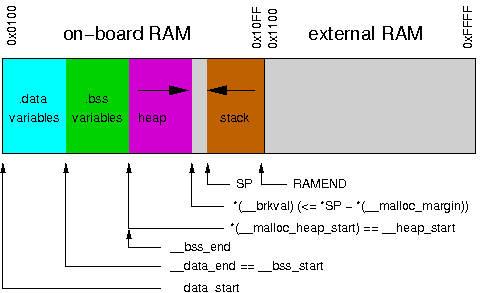
\includegraphics[width=300px]{images/malloc-std.png}
	\caption{Sections}
	\label{fig:sections}
\end{figure}

Der Anfang des Heaps wird über das Linker Script an den Compiler/Linker übergeben. Die Start-Adresse kann über die Variable \lstinline$__heap_start$ abgefragt werden.

\begin{lstlisting}[title=memory.c]
// Defined from linker script
extern char __heap_start;
char *heapStart = &__heap_start;
\end{lstlisting}

Der allozierte Speicher wird durch die \lstinline$memoryArea$ Struktur verwaltet. 

\begin{lstlisting}[title=memory.c]
typedef struct memoryArea {
    uint8_t size;
    struct memoryArea *next;
} memoryArea;
\end{lstlisting}

Vor jedem angeforderten Speicherbereich wird die Größe dieses Speicherbereichs (Variable size) abgelegt. Dadurch weiß \lstinline$freeMemory()$, wie viel Byte freigegeben werden müssen. Die Variable next erfüllt zwei Zwecke. Bei erfolgreicher Reservierung ist dies die Speicheradresse, die dem Benutzer zurück gegeben wird. Beim Freigeben des Speichers wird dieser Pointer für die verkettete List der Free-List verwendet. Der Vorteil dieses System ist, dass keine separaten Listen benötigt werden, um die Kontrollinformationen zu speichern. Die einzige Restriktion stellt die size Variable dar. Da vor jedem Speicherbereich die Größe gespeichert wird, ist der Overhead pro Speicherreservierung die Größe dieser Variable (1 Byte). \\

Bild \ref{fig:memory} verdeutlicht diesen Zusammenhang nochmals. Es sind drei Speicherblöcke (vom Typ memoryArea) abgebildet. Der mittlere (blaue) Speicherblock wurde vom Benutzer reserviert und ist in Benutzung, die beiden grünen Speichblöcke wurde wieder freigegen und befinden sich in der Free List. In jedem Speicherbereich sind die Variablen \lstinline$size$ und \lstinline$next$ abgebildet (benötigt für die Kontrollinformationen). Beim reservieren des Speicherblocks blau wurde die Adresse der Variable next an den Benutzer gegeben. Die einzige Kontrollinformation stellt die Variable \lstinline$size$ (= 20Byte) dar. In der Free List befinden sich zwei Elemente, die Variable \lstinline$next$ zeigt jeweils auf den nächsten Eintrag der Free List.

\begin{figure}[H]
	\centering
	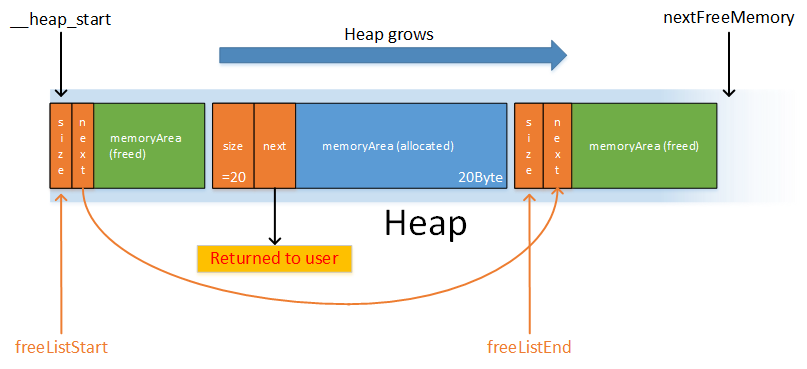
\includegraphics[width=450px]{images/memory.png}
	\caption{Dynamische Speicherverwaltung}
	\label{fig:memory}
\end{figure}

Beim reservieren von Speicher wird zunächst der verfügbare Speicher sowie auf Stack-Kollision geprüft. Kann Speicher reserviert werden, wird die Adresse des nächsten verfügbaren Speichers auf ein Pointer auf eine \lstinline$memoryArea$ Struktur gecastet. Anschließend wird die Größe des Speicherbereichs gesetzt sowie die nächste freie Speicheradresse berechnet. Die Funktion gibt die Adresse der next Variable an den Benutzer als benutzbaren Speicher auf dem Heap zurück.

\begin{lstlisting}[title=memory.c]
newMemoryArea = (memoryArea *) nextFreeMemory;
newMemoryArea->size = size;

nextFreeMemory += size + sizeof(uint8_t);

// ...

return &(newMemoryArea->next);
\end{lstlisting}

Freigegebener Speicher wird in der Free-List verwaltet. Die Free-List besteht aus einer verketteten Liste von \lstinline$memoryArea$ Elementen. Bei der Speicheranforderungen wird zuerst die Free-List betrachtet. Wird ein passender Eintrag in der Free-List gefunden, wird dieser aus der Free-List entfernt und dem Benutzer zurück geliefert. Wird kein passender Eintrag gefunden, wird überprüft, ob durch ein größeres Element in der Free-List die Speicheranforderung erfüllt werden kann. Ist dies nicht der Fall, wird neuer Speicher aus dem Heap zurück geliefert.\\

Da Heap und Stack aufeinander zu wachsen, besteht hier die Gefahr einer Kollision. Um dies zu vermeiden, wird bei Speicheranforderungen auf eine Kollision überprüft. Der Heap kann nicht weiter als bis zu einem festgelegten Abstand zum Stack wachsen. Dieser Abstand bestimmt die Variable \lstinline$margin$. Ist diese Grenze erreicht, kann \lstinline$allocateMemory()$ keinen Speicher mehr allozieren und liefert 0 zurück. Obwohl es keinen freien Speicher mehr auf dem Heap gibt, kann die Anwendung weiterhin mit dem Stack (der noch margin Bytes frei hat) arbeiten und stürzt nicht ab.

Um race-conditions zu vermeiden und die Speicherverwaltung vor Interrupts zu schützen, werden beim allozieren und freigeben Interrupts gesperrt.

\section{Verbesserungsmöglichkeiten}
Eine Verbesserungsmöglichkeit der Speicherverwaltung wäre eine Funktion zum defragmentieren des Speichers. Durch häufiges allozieren und freigeben von Speicher unterschiedlicher Größe kann es zu Fragmentierung und Speicherbrauch kommen. Zusätzlich zum Defragmentieren kann ein Buddy-System implementiert werden, welches durch aufsplitten und mergen von Speicherbereichen noch effektiver arbeiten kann.

\chapter{Message System / Shell}
\label{chap:die-shell}
Zur seriellen Kommunikation wird die USART Schnittstelle des XMega verwendet. Das Senden und Empfangen erfolgt Interrupt-gesteuert. Ein Message System wurde implementiert, um einfach Nachrichten über USART senden und empfangen zu können. Um zu verhindern, dass Messages verloren gehen oder Buffer überlaufen, wird die dynamische Speicherverwaltung zum verwalten der Messages und Queues verwendet. Eine Shell ermöglicht das komfortable Kommunizieren mit dem XMeaga über USART. Die Shell läuft als eigener Task und wird wie alle Tasks geschedult.\\

Zum Verwalten der USART Nachrichten werden verschiedene Buffer verwendet, welche in der Dateien \lstinline$usart_message.h$ und \lstinline$usart_queue.h$ deklariert sind.

\section{Message Queues}
\label{subsec:shell-queue}
Zum Empfangen und Senden werden Message Queues (verkettete Listen) vom Typ \lstinline$messageQueue$ verwendet.\\

\begin{lstlisting}
struct messageQueue
{
	message *tail;
	message *head;
	int size;
};
\end{lstlisting}

Zum Erzeugen und Zerstören von Message Queues werden die Funktionen

\begin{lstlisting}
messageQueue *getMessageQueue();
void destroyMessageQueue(messageQueue *queue);
\end{lstlisting}

verwendet. Diese verwenden intern zum Reservieren/Freigeben des Speichers der Queue die dynamische Speicherverwaltung. Beim Freigeben des Speichers der Queue wird auch der Speicher aller Elemente in der Queue freigegeben.\\

Zum Hinzufügen und Auslesen von Messages aus einer Queue werden die Funktionen

\begin{lstlisting}
void enqueue(messageQueue *queue, message *msg);
message *dequeue(messageQueue *queue);
\end{lstlisting}

benutzt. Wichtig ist, dass die übergebene Message nach einem Aufruf von \lstinline$enqueue()$ von der Message Queue verwaltet wird und keine Kopie dieser Message gemacht wird. Es wird kein Aufruf von \lstinline$destroyMessage()$ für die übergebene Message benötigt.

\section{Messages}
\label{subsec:shell-messages}
Um Daten zu senden und zu empfangen werden Messages verwendet.\\

\begin{lstlisting}
struct message
{
	char *data;
	int size;

	int stackIndex;
	MSG_TYPE type;

	message *next;
};
\end{lstlisting}

Die Variable type bestimmt dabei, ob die Art des Messages.
\begin{itemize}
	\item TX\_MSG: Messages um über USART zu senden.
	\item RX\_MSG: Messages um über USART zu empfangen.
\end{itemize}

Die Variable stackIndex wird verwendet, um eine Message als Stack benutzen zu können. je nach MSG\_TYPE können Byte-weise Daten gepusht oder gepopt werden. Dies erlaubt ein komfortables Senden und Empfangen bei der USART Kommunikation, da über USART immer nur 1 Byte gesendet/empfangen werden kann. Beispielsweise kann in jedem USART data-receive interrupt jeweils ein Byte auf die aktuelle Message gepusht werden. Es entfällt das manuelle Berechnen des nächsten freien Bytes in der Message. Um Daten zu Senden, können je nach bedarf verschiedene Funktionen benutzt werden.\\

Wie bei Message Queues gibt es jeweils eine Funktion zum erzeugen und zerstören von Messages. Es wird ebenfalls die dynamische Speicherverwaltung verwendet. \lstinline$getMessage()$ bekommt als Parameter die Größe der Message in Bytes, sowie den Message Typ, welcher den Stack-Zugriff vorgibt.\\

\begin{lstlisting}
message *getMessage(int dataSize, MSG_TYPE type);
void destroyMessage(message *msg);
\end{lstlisting}

Zum setzen des Inhalts der Message wird \lstinline$setMessageData()$ verwendet. Die übergebenen Daten werden dabei in den Message Buffer kopiert.\\

\begin{lstlisting}
int setMessageData(message *msg, char *data, int size);
\end{lstlisting}

Um die Daten einer Message auszulesen werden die folgenden Funktionen verwendet:\\

\begin{lstlisting}
char getMessageDataCopy(message *msg, char **data, int *size);
char *getMessageData(message *msg);
\end{lstlisting}

\lstinline$getMessageDataCopy()$ liefert eine Kopie der Daten zurück (char **data). Das bedeutet, diese Daten müssen nach Benutzung mit \lstinline$freeMemory()$  freigegeben werden. \lstinline$getMessageData$ liefert einen Pointer auf die Daten der Message zurück. Dieser Speicher darf nicht mit \lstinline$freeMemory()$  freigegeben werden. Auch muss beim Zugriff auf diese Adresse sichergestellt sein, dass die dazugehörige Message noch nicht gelöscht wurde. Wird eine Kopie einer Message inklusive Daten benötigt kann folgende Funktion verwendet werden:\\

\begin{lstlisting}
message *copyMessage(message *msg);
\end{lstlisting}

Vorgang zum Erzeugen von Messages:\\

\begin{lstlisting}
char character = '\n';
message *msg;

msg = getMessage(1, TX_MSG);
if (msg == 0)
	error();
	
setMessageData(msg, &character, 1);

// Use message

destroyMessage(msg);
\end{lstlisting}

\section{USART Kommunikation}
\label{subsec:shell-communication}
Die Datei \lstinline$usart.h$ bietet Funktionen zum Initialisieren der USART-Schnittstelle sowie zum Senden und Empfangen von Messages. Um direkt Messages zu empfangen/senden werden folgende Funktionen verwendet:\\

\begin{lstlisting}
void sendMessageUsart(message *msg);
message *receiveMessageUsart();
\end{lstlisting}

Jede Empfangene Message besteht aus einem Null-terminierten String. Nach einem Aufruf von \lstinline$sendMessageUsart()$ wird die Message vom USART System verwaltet. Der Benutzer sollte nicht mehr auf die Message zugreifen. Für die Verwaltung (Speicher freigeben) der zurückgelieferten Message von \lstinline$receiveMessageUsart()$ ist der Benutzer selbst zuständig. Zusätzlich können zum Senden von Strings komfortablere Funktionen verwendet werden. Der Benutzer muss hierbei selbst keine Messages erzeugen.\\

\begin{lstlisting}
void print(char *string);
void printChar(char character);
\end{lstlisting}

\lstinline$print$ erwartet als Paramter einen Null-terminierten String, welcher in den internen Buffer kopiert wird.

\section{USART Kommunikation Implementierung}
\label{subsec:shell-communication-impl}
Die USART Kommunikation erfolgt Interrupt-gesteuert. Folgender Frame Format wird verwendet:\\

\lstinline$Asynchronous Communicatin Mode, no parity, 1 Stop Bit, 8 Bit data$\\

Als Standard-Wert ist eine Baudrate von 115200 eingestellt. Baudrate und USART Geräte können über die folgenden Defines eingestellt werden:\\

\begin{lstlisting}
#define USART USARTC0
#define USART_PORT PORTC
#define BAUDRATE 115200
\end{lstlisting}

Zum Senden und Emfangen werden Low-Level Interrupts verwendet. Wurde ein Byte empfangen, wird der USARTC0\_RXC\_vect Interrupt getriggert. Können Daten in den USART hardware Buffer kopiert werden, wird der USARTC0\_DRE\_vect Interupt getriggert (data register empty). Empfangene und zu sendende Messages werden in Message Queues gespeichert. Da das Message System mit dynamischer Speicherverwaltung arbeitet, können keine Messages verloren gehen.\\

\begin{lstlisting}
static messageQueue *rxQueue;
static messageQueue *txQueue;
\end{lstlisting}

Der Zugriff auf die Message Queues wird durch Interrupt-sperren gesichert, da von Tasks sowie von Interrupts auf diese zugegriffen wird. Beide USART Interrupts arbeiten auf dem System Stack.

\subsection{Empfangen von Messages}
Es werden so lange Bytes empfangen und in die Message \lstinline$currentReceiveMessage$ gepusht, bis eine neue Zeile erkannt wurde oder eine bestimmte maximale Länge der Message (\lstinline$MAX_RECEIVE_MSG_SIZE$) erreicht wurde. Erst dann wird eine Message in die receive queue hinzugefügt und es wird eine neue \lstinline$currentReceiveMessage$ erzeugt. Die Empfangsroutine prüft zusätzlich auf verschiedene escape Sequenzen wie DEL, CR, ESC, usw,. Um zu verhindern dass der command prompt gelöscht werden kann wird bei DEL die cursor position abgefragt. Verschiedene Funktionen garantieren, dass die empfangene Message immer nur die minimale Größe besitzt. Bild \ref{fig:usart_receive} zeigt den groben Ablauf beim Empfangen von Nachrichten.

\begin{figure}[H]
	\centering
	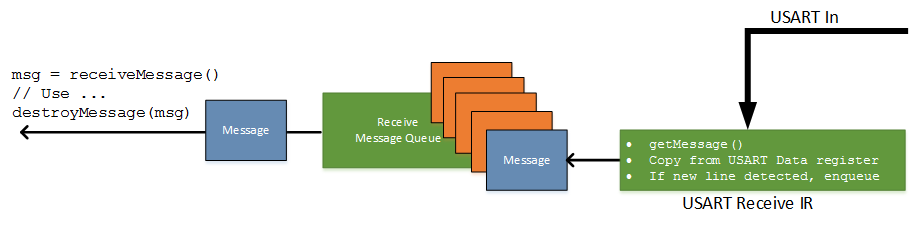
\includegraphics[width=450px]{images/UsartIn.png}
	\caption{USART Receive}
	\label{fig:usart_receive}
\end{figure}

\subsection{Senden von Messages}
Senden erfolgt analog zum Empfangen. Die variable \lstinline$currentSendMsg$ enthält die gerade zu sendende Message. Im DRE Interrupt wird immer 1 Byte von dieser Message gepopt. Wurde diese vollständig gesendet kann der Speicher der Message freigegeben werden und es kann die nächste Message aus der send queue gesendet werden. Der DRE Interrupt wird aktiviert, sobald eine Nachricht gesendet werden soll. Wurden alle Nachrichten aus der Queue gesendet, wird dieser deaktiviert. Bild \ref{fig:usart_send} zeigt das Versenden von Nachrichten.

\begin{figure}[H]
	\centering
	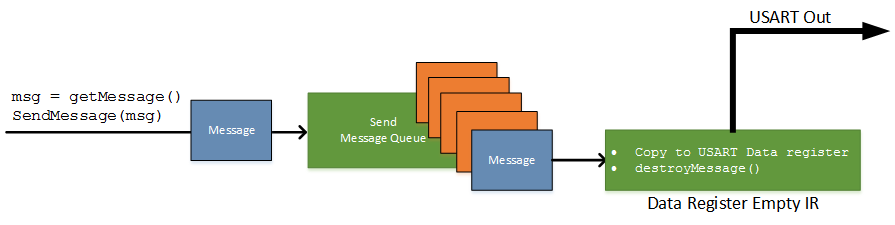
\includegraphics[width=450px]{images/UsartOut.png}
	\caption{USART Send}
	\label{fig:usart_send}
\end{figure}

\section{Shell Task}
\label{subsec:shell-task}
Die Shell Tasks wird wie alle anderen Tasks geschedult und verarbeitet und interpretiert die empfangenen Messages. In der Headerdatei \lstinline$shell.c$ kann der command prompt der Shell konfiguriert werden. Die Funktion\\

\begin{lstlisting}
void setMessageCallback(void (*processMessageCB)(char *msg));
\end{lstlisting}

erlaubt das Setzen einer Callback-Funktion. Die Shell-Task verarbeitet die Empfangenen Daten und verarbeitet ggf. die Befehle. Alle nicht verarbeiteten Daten werden an die Callback-Funktion übergeben.

\subsection{Implementierung}
Die Funktion \lstinline$waitForMessage$ wird verwendet um aktiv auf eine Message zu warten:

\begin{lstlisting}
static message *waitForMessage()
{
    message *msg;

    while (1) {
        msg = receiveMessageUsart();
        if (msg != 0)
            break;
    }

    return msg;
}
\end{lstlisting}

Wurde eine Message empfangen wird \lstinline$parseMessage$ aufgerufen, welche die Message verarbeitet. Folgende befehle sind verfügbar:

\begin{itemize}
	\item ledOn Schaltet die led1 an
	\item ledOff Schaltet die led1 aus
	\item memDump Gibt Informationen der dynamischen Speicherverwaltung aus
\end{itemize}

%\begin{figure}[H]
%	\centering
%	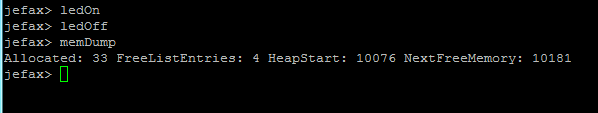
\includegraphics[width=450px]{images/shell.png}
%	\caption{jefax shell}
%	\label{fig:shell}
%\end{figure}

\chapter{Fazit}
\label{chap:fazit}

Jefax bietet eine gute Möglichkeit Tasks quasi-parallel auf einem XMega ablaufen zu lassen. Jedoch werden atomare Zugriffe und der gegenseitige Ausschluss durch viele Interruptsperren realisiert. Dadurch hat das System eine hohe Interruptlatenzzeit, was vor allem in Realzeitsystemen beachtet werden muss.
Das Timer Framework von Jefax wird durch einen Hardware Interrupt realisiert. Somit laufen alle Timer Callbacks im Interruptkontext. Dies verlangt einen gewissen Grad an Erfahrung und Aufmerksamkeit des Nutzers. Intuitiver und weniger fehleranfällig wäre eine Realisierung als Softinterrupt.
Die Realisierung des Schedulers als struct bietet eine hohen Grad an Erweiterbarkeit und Flexibilität. Jedoch kann durch einen fehlerhaft implementierten Scheduler das komplette System lahmgelegt und untergraben werden.

\begin{thebibliography}{999}
\bibitem{bib-memory} \url{http://www.nongnu.org/avr-libc/user-manual/malloc.html}
\end{thebibliography}

\cleardoublepage
\addcontentsline{toc}{chapter}{\listfigurename}
\listoffigures

\end{document}